\section{Background and Motivation}
\label{sec:background-motivation}

In this section, we motivate our research by outlining a few concrete real-world

\subsection{Motivating Applications}
\label{sec:motiv-appl}

Background on wide area streaming analytics; Application examples

We consider three distinct area, yet architecturally similar applications. These
applications represent the streaming applications that span the wide area and
the traditional ways have been aggregating them and processing offline.

\begin{figure}
  \centering
  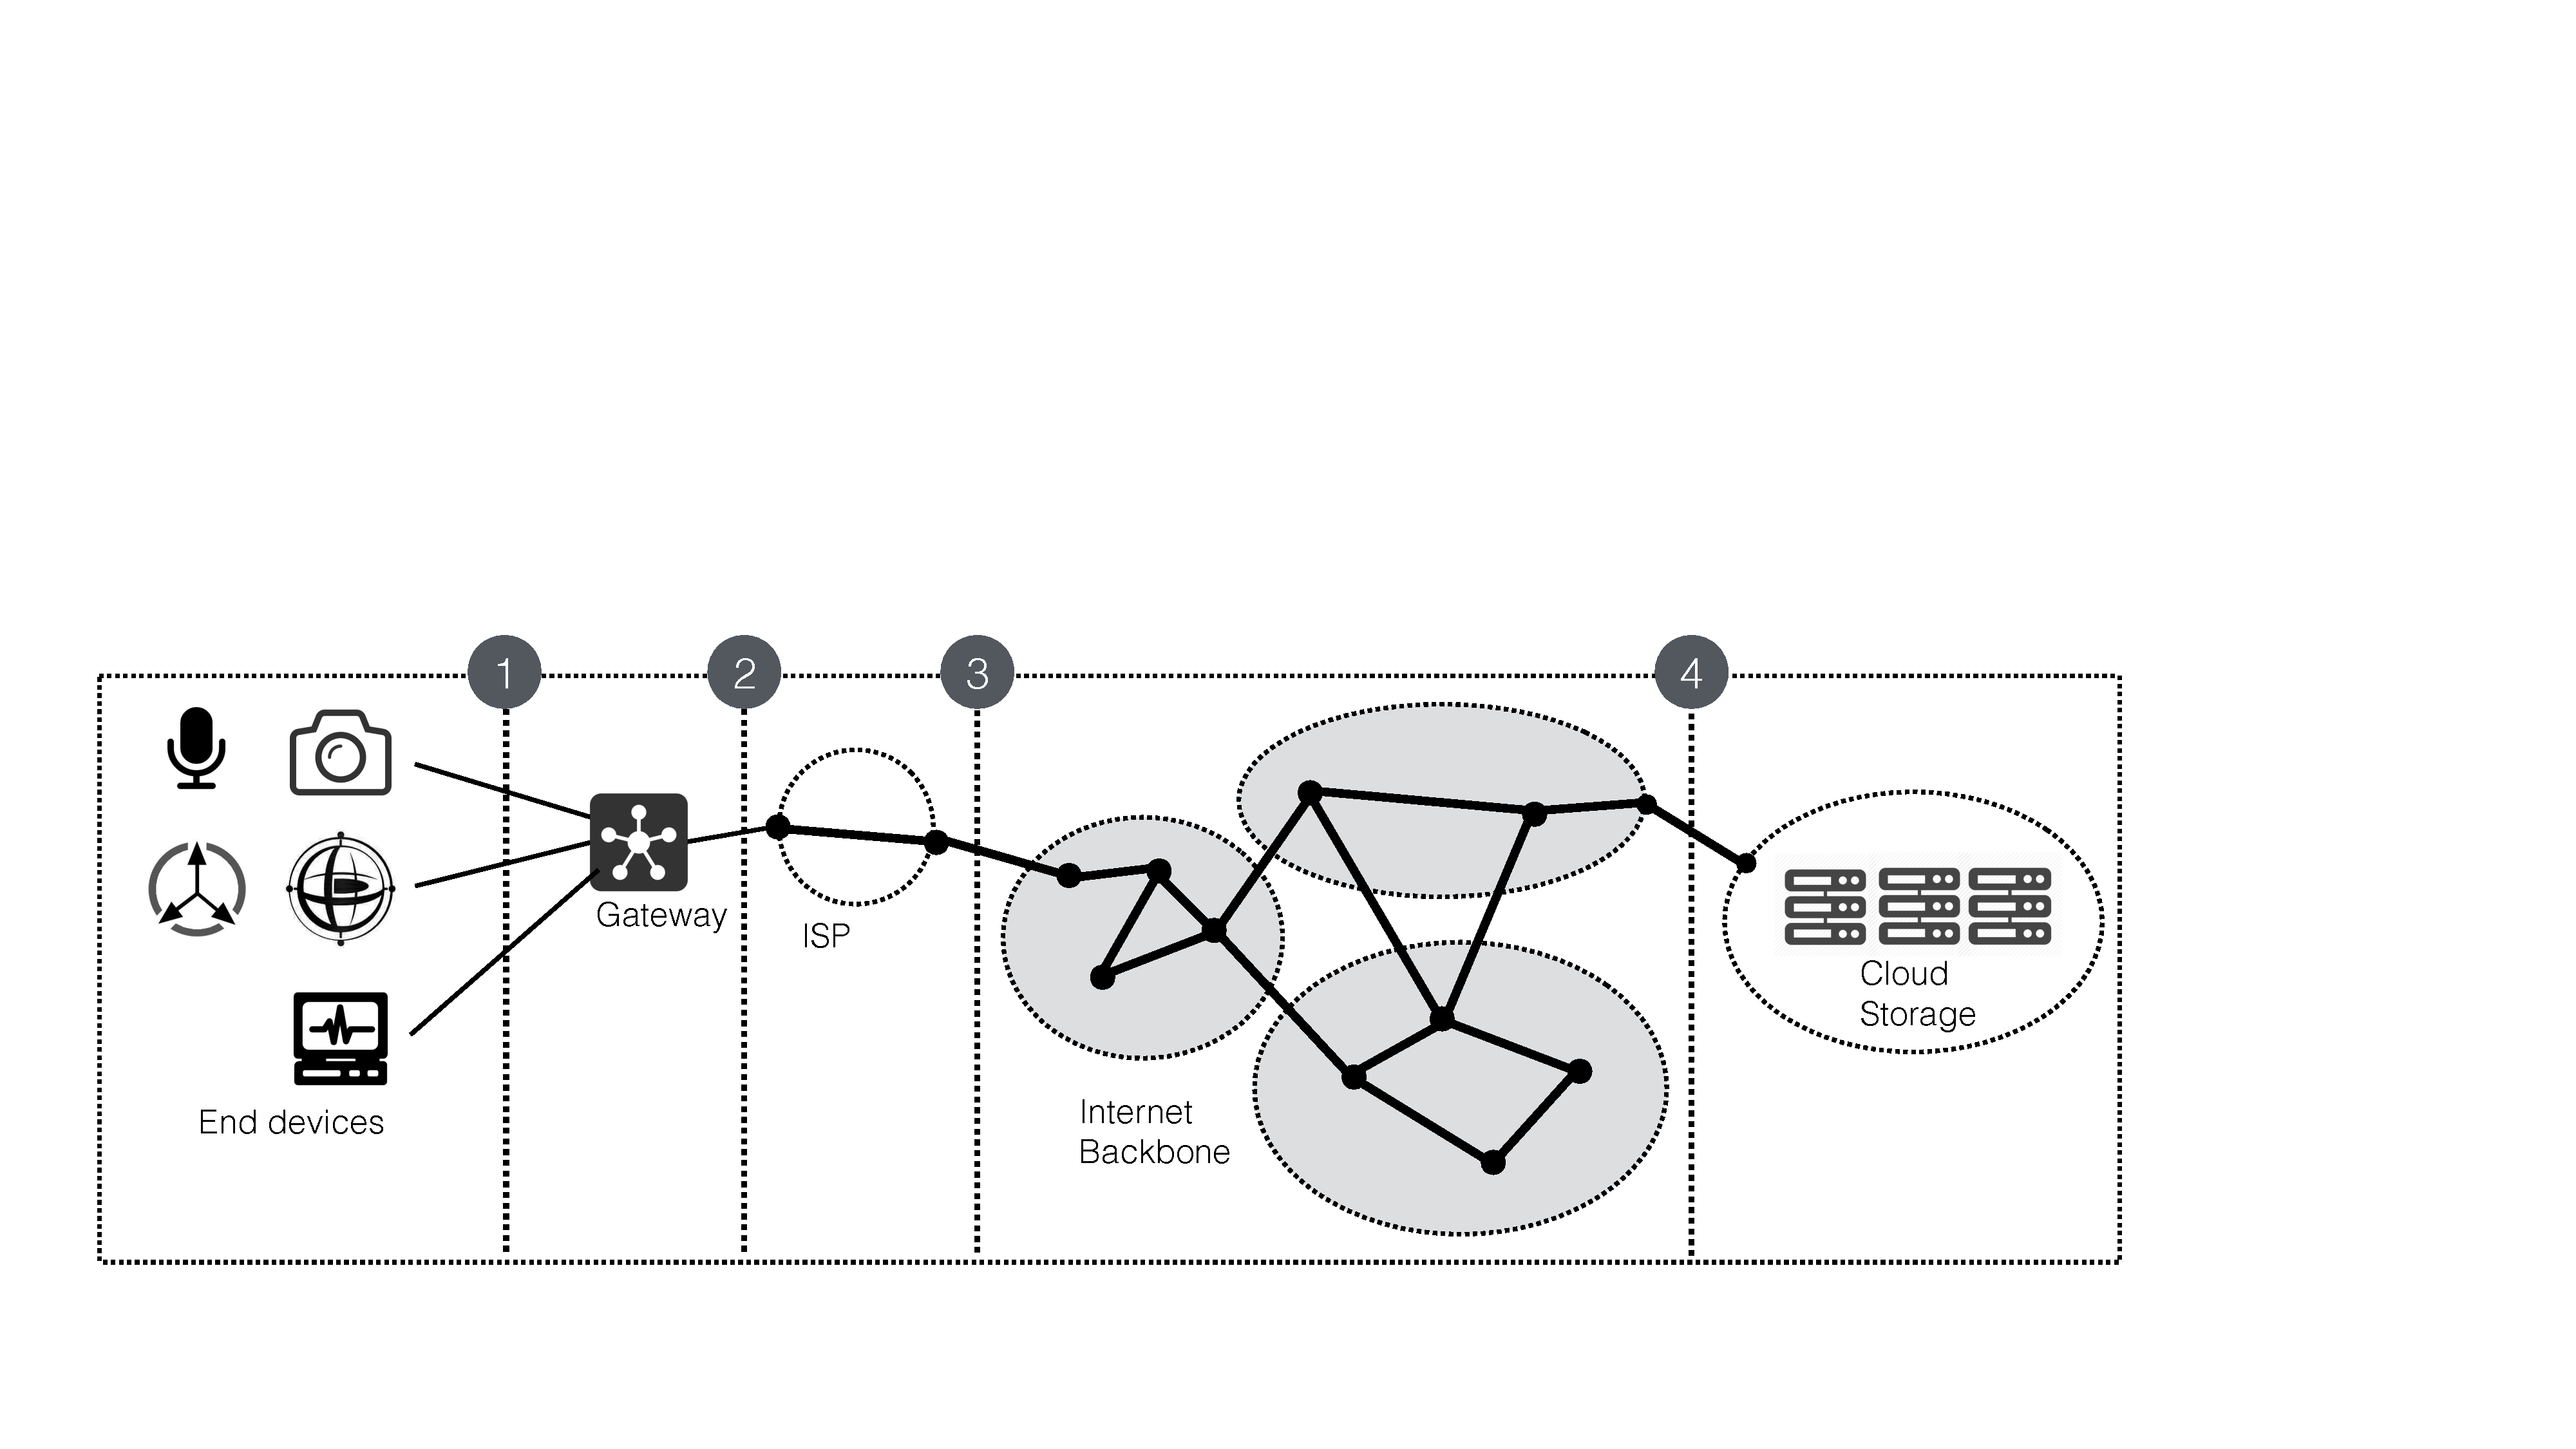
\includegraphics[width=.95\linewidth]{figures/model.pdf}
  \label{fig:app-model}
  \caption{Stream Processing Applications}
\end{figure}

\subsubsection{Smart City}
\label{sec:smart-city}

\todo{ask for Shenzhen's data}

\subsubsection{Continuous Visual Event Recognition}
\label{sec:cont-visu-event}

We use VIRAT Video Dataset~\cite{oh2011large} and count the number of people in
each frame. Such application can be useful in retail stores or large shopping
malls.

\subsubsection{Log Monitoring}
\label{sec:log-monitoring}

\todo{Conviva Log}.

\subsection{Making the Case for Adaptive Execution}
\label{sec:making-case-adapt}

In this section, we characterize the resource availability in the wide-area. To
understand the real-world characteristics, we've conducted some measurements
using computers at the edge as well as in the cloud.

Our key take-away is that the latency is mostly stable but the available
bandwidth has large variation, even in well-provisioned connections that one
would assume between Amazon data centers.

\begin{figure}
  \centering
  \begin{subfigure}{.48\columnwidth}
    \centering
    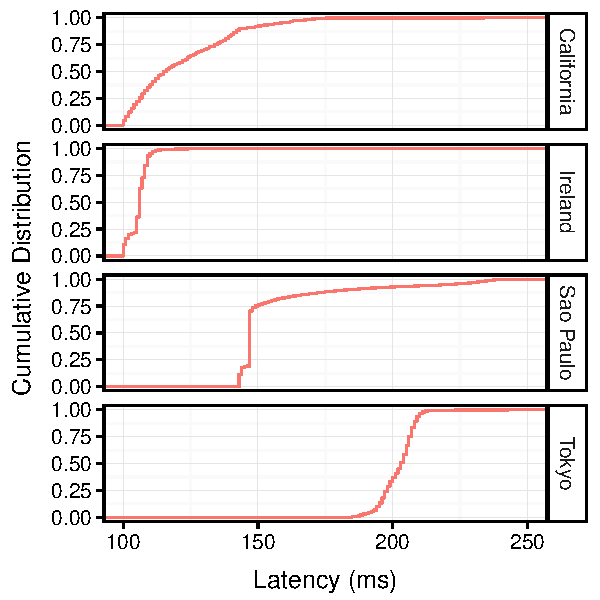
\includegraphics[width=.95\linewidth]{figures/latency-cdf.pdf}
    \caption{CDF}
    \label{fig:bar}
  \end{subfigure}
  \begin{subfigure}{.48\columnwidth}
    \centering
    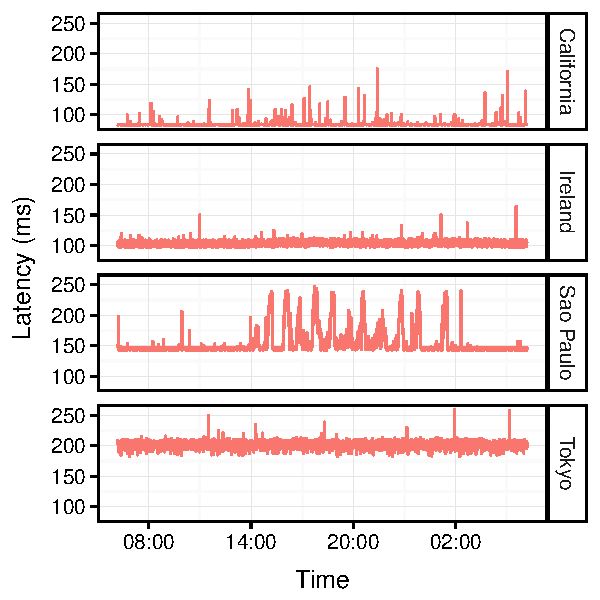
\includegraphics[width=.95\linewidth]{figures/latency-ts.pdf}
    \caption{Timeseries plot}
    \label{fig:ts}
  \end{subfigure}
  \caption{Latency measurement between U.S. west and other EC2 sites. Data from Bailis~\cite{bailis2013highly}.}
  \label{fig:bw}
\end{figure}

\begin{figure}
  \centering
  \begin{subfigure}{.48\columnwidth}
    \centering
    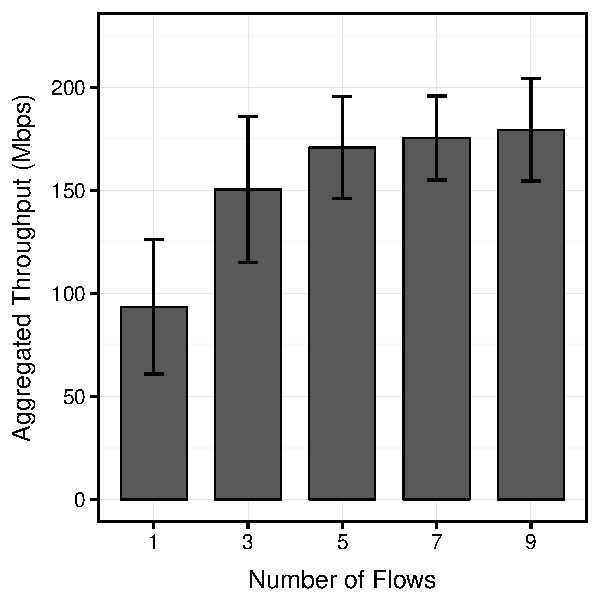
\includegraphics[width=.95\linewidth]{figures/bw-bar.pdf}
    \caption{Bar plot}
    \label{fig:bar}
  \end{subfigure}
  \begin{subfigure}{.48\columnwidth}
    \centering
    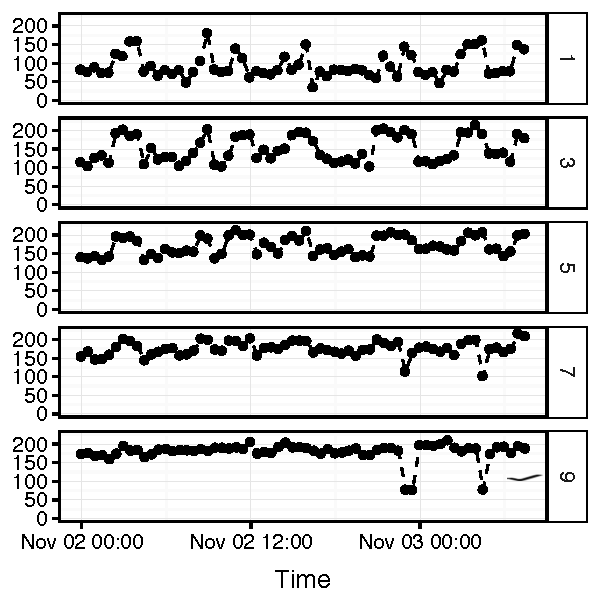
\includegraphics[width=.95\linewidth]{figures/bw-ts.pdf}
    \caption{Timeseries plot}
    \label{fig:ts}
  \end{subfigure}
  \caption{Bandwidth fluctuations from Europe EC2 (Ireland) to US-East
    (Virginia)}
  \label{fig:bw}
\end{figure}

Application can transmit a large chunk of data if needed. But when the network
condition deteriorate, doing so will create back-logged data. Not all sensor
data and log data are inheritantly important, many application can tolerate data
loss. So we could degrade the data quality but remains responsive.

\subsection{PAR Tradeoff}
\label{sec:par-tradeoff}

When fixed resource, often the accuracy and performance needs trade-off.

\begin{figure}
  \centering
  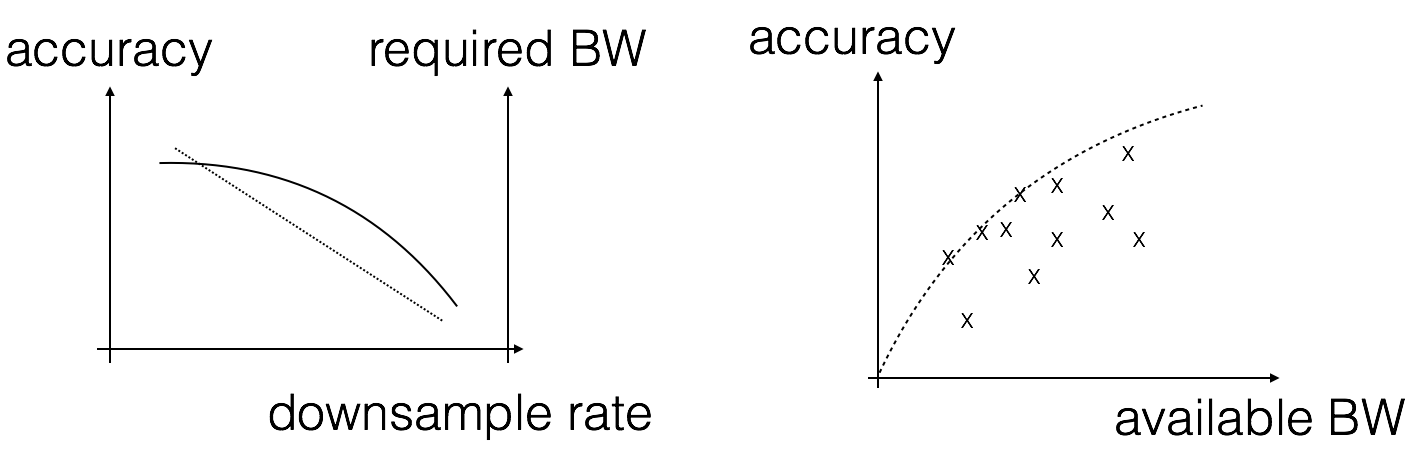
\includegraphics[width=.95\linewidth]{figures/tradeoff-placeholder.png}
  \caption{Expected Trade-off between application requirement and BW}
  \label{fig:degrade}
\end{figure}

\begin{figure}
  \centering
  \begin{subfigure}{.42\columnwidth}
    \centering
    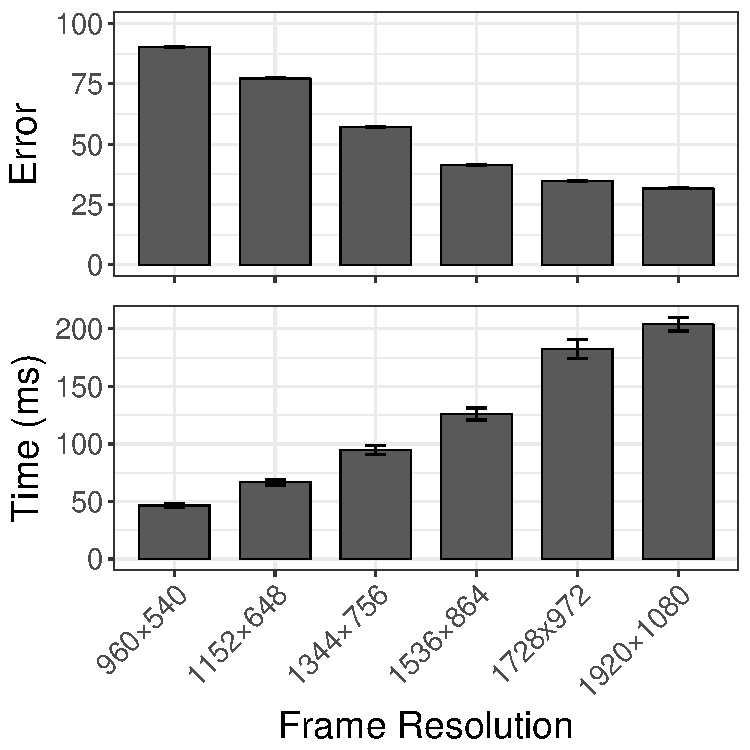
\includegraphics[width=.90\linewidth]{figures/accuracy-performance.pdf}
    \label{fig:a-vs-p}
  \end{subfigure}
  \begin{subfigure}{.54\columnwidth}
    \centering
    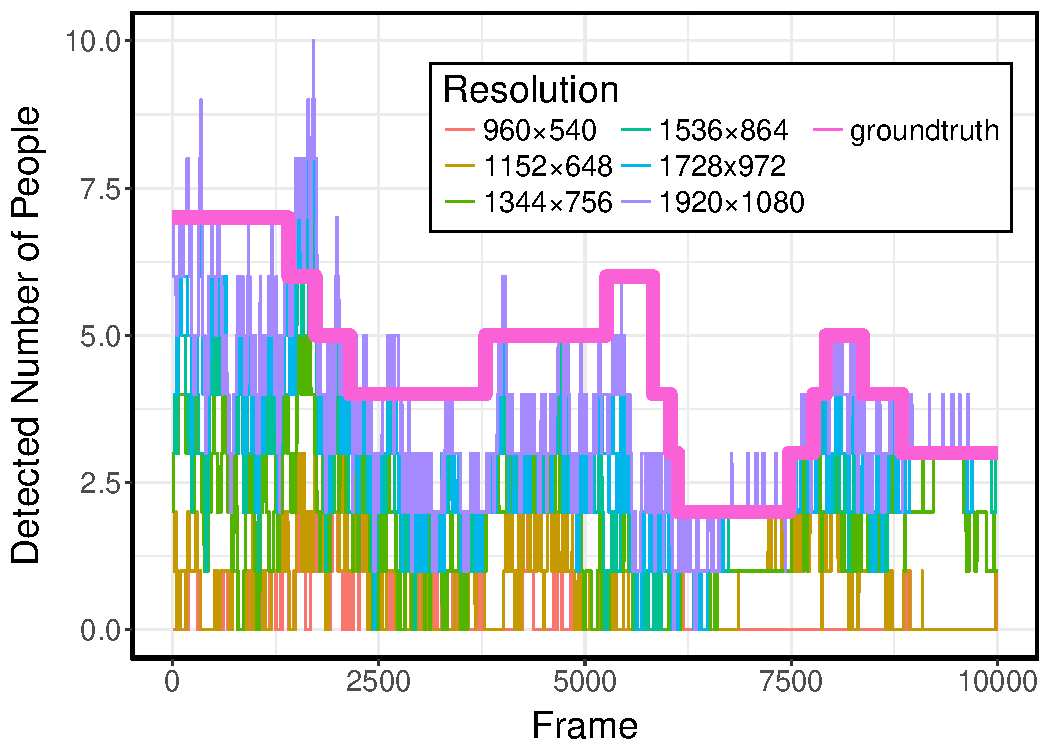
\includegraphics[width=.95\linewidth]{figures/time-series.pdf}
    \label{fig:detect-ts}
  \end{subfigure}
  \caption{Accuracy and Performance Trade off}
  \label{fig:bw}
\end{figure}

%% Maybe also last hop wireless?

%%% Local Variables:
%%% mode: latex
%%% TeX-master: "sigcomm2017"
%%% End:
